
\chapter[Global System For Mobile Communications]{Global System For Mobile Communications (GSM)}
\gls{gsm} is the most successful digital mobile telecommunication system in the world. It is used by billions of people around the world.

In the early 1980s, Europe had numerous coexisting analog mobile phone systems, which were often based on similar standards, but ran on slightly different carrier frequencies. To avoid this situation for a second generation fully digital system, the \textbf{groupe spéciale mobile (GSM)} was founded in 1982. This system was soon named the \textit{global system for mobile communications (GSM}), with the specification process lying in the hands of \gls{etsi}. 

The primary goal of \gls{gsm} was to provide a mobile phone system that allows users to roam throughout Europe and provides voice services compatible to \gls{isdn} and other \gls{pstn} systems.

\begin{itemize}
	\item \gls{gsm} is a typical second generation system, replacing the first generation analog systems. 
	\item \gls{gsm} has initially been deployed in Europe using 890–915 MHz for uplinks and 935–960 MHz for downlinks.
	\item There are multiple versions of \gls{gsm} system.
		\begin{itemize}
			\item \textbf{GSM 900}: GSM at 900 MHz.
			\item \textbf{Digital Cellular Service (DCS)} 1800: GSM at 1800 MHz.
			\item \textbf{Personal Communication Service (PCS) 19000}: GSM at 1900 MHz.	
		\end{itemize}
\end{itemize}


\section{Mobile Services}
\gls{gsm} permits the integration of different voice and data services and the interworking with existing networks. Services make a network interesting for customers. \gls{gsm} has defined three different categories of services: 
\begin{itemize}
	\item bearer services
	\item tele services and
	\item supplementary services
\end{itemize}

%%%%%%%%%%%%%%%%%%%%%%%%%%%%%%%%%%%%%%%%%%%%%%
%				
%				Figure
%
%%%%%%%%%%%%%%%%%%%%%%%%%%%%%%%%%%%%%%%%%%%%%%

%\begin{figure}[h]
%	\centering
%	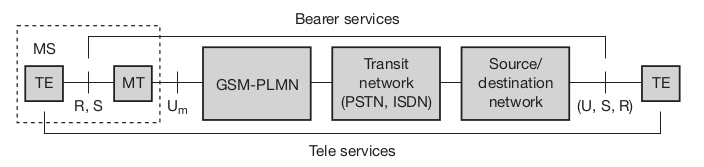
\includegraphics[width=0.8\textwidth]{bearer-and-tele-services}
%	\caption{Bearer and tele services reference model}\label{fig:bearer-and-tele-services}
%\end{figure}

%Figure \ref{fig:bearer-and-tele-services} shows a reference model for GSM services. A \textbf{mobile station MS} is
%connected to the \textbf{GSM public land mobile network (PLMN)} via the $ U_m $ interface. (GSM-PLMN is the infrastructure needed for the GSM network.) This
%network is connected to transit networks, e.g., \textbf{integrated services digital network (ISDN)} or traditional \textbf{public switched telephone network (PSTN)}. There
%might be an additional network, the source/destination network, before another
%\textbf{terminal TE} is connected. \textbf{Bearer services} now comprise all services that enable
%the transparent transmission of data between the interfaces to the network, i.e., $ S $
%in case of the mobile station, and a similar interface for the other terminal (e.g.,
%$ S_0 $ for ISDN terminals). Interfaces like $ U $, $ S $, and $ R $ in case of ISDN have not been
%defined for all networks, so it depends on the specific network which interface is
%used as a reference for the transparent transmission of data. In the classical GSM
%model, bearer services are connection-oriented and circuit- or packet-switched.
%These services only need the lower three layers of the ISO/OSI reference model.
%
%Within the mobile station MS, the \textbf{mobile termination (MT)} performs all
%network specific tasks (TDMA, FDMA, coding etc.) and offers an interface for
%data transmission (S) to the terminal TE which can then be network indepen-
%dent. Depending on the capabilities of TE, further interfaces may be needed,
%such as $ R $, according to the ISDN reference model. Tele services
%are application specific and may thus need all seven layers of the ISO/OSI refer-
%ence model. These services are specified end-to-end, i.e., from one terminal TE
%to another.

\subsection{Bearer Services}
Bearer services are telecommunication services that are used to transfer user data and control signals between two pieces of equipment.
Bearer services permit 
 \begin{itemize}
 	\item transparent and non-transparent, 
 	\item synchronous or asynchronous data transmission. 
 \end{itemize}

 
 \subsubsection*{Transparent Bearer Services}
 \begin{itemize}
 	\item Transparent bearer services only use the functions of the physical layer (layer 1) to transmit data. 
 	\item Data transmission has a constant delay and throughput if no transmission errors occur.
 	\item Transparent bearer services do not try to recover lost data.
 \end{itemize}

\subsubsection*{Non-transparent Bearer Services}
Non-transparent bearer services use protocols of layers two and three to implement error correction and flow control.

\subsection{Tele services}
\gls{gsm} mainly focuses on voice-oriented tele services. These comprise encrypted voice transmission, message services, and basic data communication with terminals as known from the \gls{pstn} or \gls{isdn}. 

%\subsection*{GSM Tele Services}

\subsubsection{Telephony}
The primary goal of GSM was the provision of high-quality digital voice transmission.

\subsubsection{Emergency Number}
This service is mandatory for all providers and free of charge. This connection also has the highest priority, possibly pre-empting other connections, and will automatically be set up with the closest emergency center.

\subsubsection{SMS}
\gls{sms} offers transmission of messages of up to 160 characters. It's successor is \gls{ems}.

\subsubsection{EMS}
\gls{ems} offers a \textit{larger message size} (e.\ g.\ , 760 characters), \textit{formatted text}, and the \textit{transmission of animated pictures}, \textit{small images} and \textit{ring tones} in a standardized way. 

\subsubsection{MMS}
EMS never really took off. \gls{mms} offers the transmission of \textit{larger pictures}, \textit{short video clips} etc. 

\subsubsection{Group 3 Fax}
Group 3 fax is a non-voice tele service. Fax data is transmitted as digital data over the analog telephone network using modems. 


\subsection{Supplementary services}
In addition to tele and bearer services, GSM providers can offer \textbf{supplementary services}. These services offer various enhancements for the standard telephony service. Typical services are:

\begin{multicols}{2}
	\begin{itemize}
		\item user identification
		\item call redirection
		\item closed user groups and 
		\item multi party communication
	\end{itemize}
\end{multicols}

Closed user groups allow, for example, a company-specific \gls{gsm} sub-network, to which only members of the group have access.

\section{System Architecture}
Figure \ref{fig:gsm-architecture} gives an overview of the \gls{gsm} system. A \gls{gsm} system consists of three subsystems:
%\begin{enumerate}
%	\item \textbf{the radio subsystem (RSS)}
%	\item \textbf{the network and switching subsystem (NSS)} and
%	\item \textbf{the operation subsystem (OSS)}
%\end{enumerate}
\begin{enumerate}
	\item \textit{\gls{rss}}
	\item \textit{\gls{nss}} and
	\item \textit{\gls{oss}}
\end{enumerate}

\begin{framed}
\begin{nepali}
\noindent नाेटः GSM Architecture with interface भनेमा Figure \ref{fig:gsm-architecture} मा देखाइएकाे सबै बनाउने।
\end{nepali}
\end{framed}


%%%%%%%%%%%%%%%%%%%%%%%%%%%%%
%							%
%		Chapters			%
%							%
%%%%%%%%%%%%%%%%%%%%%%%%%%%%%
\begin{figure}[hb!]
	\centering
	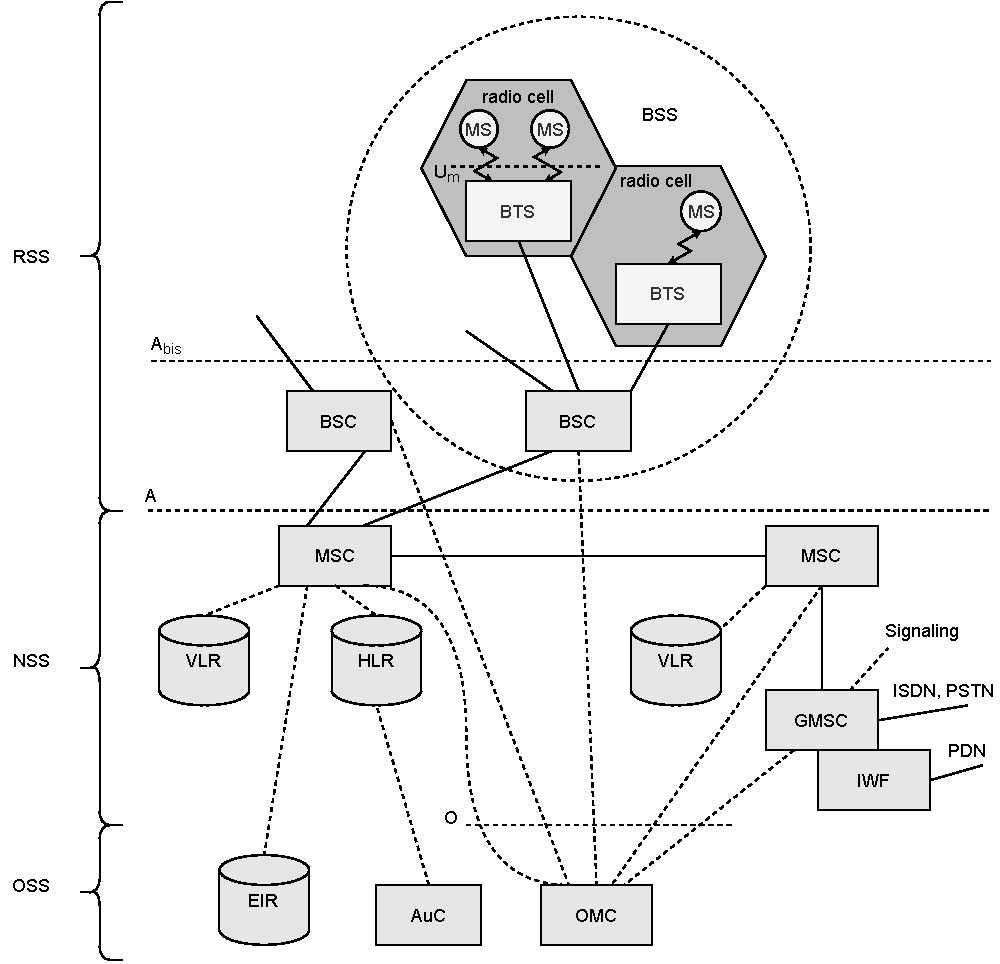
\includegraphics[width=0.8\textwidth]{gsm-architecture.pdf}
	\caption{Functional architecture of a GSM system}\label{fig:gsm-architecture}
\end{figure}

\subsection[Radio Subsystem]{Radio Subsystem (RSS)}
\begin{itemize}
	\item \gls{rss} comprises all radio specific entities, i.\ e.\,  \textit{\gls{ms}} and \textit{\gls{bss}}.
	\item Figure \ref{fig:gsm-architecture} shows the connection between the \gls{rss} and the \gls{nss} via the  \textbf{A interface} (solid lines) and the connection to the \gls{oss} via the \textbf{O interface} (dashed lines).
\end{itemize}


\subsubsection[BSS]{Base Station Subsystem (BSS)}
\begin{itemize}
	\item A \gls{gsm} network comprises many \gls{bss}s, each controlled by a \gls{bsc}. 
	\item The \gls{bss} performs all functions necessary to maintain: 
	\begin{itemize}
		\item radio connections to an \gls{ms}, 
		\item coding/decoding of voice, and 
		\item rate adaptation to/from the wireless network part.
	\end{itemize}
 \item Besides a \gls{bsc}, the \gls{bss} contains several BTSs.
\end{itemize}


\subsubsection[BTS]{Base Transceiver Station (BTS)}
\begin{itemize}
	\item A \gls{bts} comprises all radio equipment, i.\ e.\ , \textit{antennas}, \textit{signal processing}, \textit{amplifiers} necessary for radio transmission. 
	\item A \gls{bts}:
	\begin{itemize}
		\item can form a radio cell using sectorized antennas.
		\item is connected to \gls{ms} via the \( U_m \) {interface}, and 
		\item connected to the \gls{bsc} via the  \(A_{bis}\)  {interface}.
	\end{itemize}
\item The $ U_m $ interface contains all the mechanisms necessary for wireless transmission.
\item A \gls{gsm} cell can measure between some \(100 m\) and \(35 km\) depending on the environment. 
\end{itemize}


\paragraph*{Tasks of The \gls{bts} Within a \gls{bss}}
\begin{multicols}{2}
	\begin{itemize}
		\item Frequency hopping
		\item Channel coding and decoding
		\item Rate adaptation
		\item Encryption and decryption
		\item Paging
		\item Uplink signal measurement
	\end{itemize}
\end{multicols}


\subsubsection[BSC]{Base Station Controller (BSC)}
\begin{itemize}
	\item The \gls{bsc} basically manages the \gls{bts}s.
	\item It \textit{reserves radio frequencies}, \textit{handles the handover} from one \gls{bts} to another within the \gls{bss}, and \textit{performs paging} of the \gls{ms}. 
	\item The \gls{bsc} also \textit{multiplexes the radio channels} onto the fixed network connections at the \(A\) interface.
\end{itemize}


\paragraph*{Tasks of The \gls{bsc} Within a \gls{bss}}
\begin{multicols}{2}
	\begin{itemize}
		\item Management of radio channels
		\item Frequency hopping
		\item Management of terrestrial channels
		\item Mapping of terrestrial onto radio channels
		\item Encryption and decryption
		\item Paging
		\item Traffic measurement
		\item Authentication
		\item Location registry, location update
		\item Handover management
	\end{itemize}
\end{multicols}



\subsubsection[MS]{Mobile Station(MS)}
\begin{itemize}
	\item The \gls{ms} comprises all user equipment and software needed for communication with a \gls{gsm} network.
	\item An \gls{ms} consists of:
	\begin{itemize}
		\item user independent hardware and software and
		\item the \textit{\gls{sim}}, which stores all user-specific data that is relevant to \gls{gsm}\footnote{Many additional items can be stored on the mobile device. However, this is irrelevant to GSM.}. 
	\end{itemize}
\item An \gls{ms} can be identified via the \textit{\gls{imei}}.
\end{itemize}

 A user can personalize any \gls{ms} using his or her \gls{sim}. The \gls{sim} card contains many identifiers and tables, such as:
\begin{multicols}{2}
	\begin{itemize}
		\item card-type 
		\item serial number
		\item a list of subscribed services
		\item a \textit{\gls{pin}}
		\item a \textit{\gls{puk}}
		\item an authentication key $  K_i $ , and 
		\item the \textit{\gls{imsi}}
	\end{itemize} 
\end{multicols}

The \gls{pin} is used to unlock the \gls{ms}. Using the wrong \gls{pin} three times will lock the \gls{sim}. In such cases, the \gls{puk} is needed to unlock the \gls{sim}. The \gls{ms} stores dynamic information while logged onto the \gls{gsm} system, such as, e.\ g.\ , the cipher key $ K_c $ and the location information consisting of a \textit{\gls{tmsi}} and the \textit{\gls{lai}}.


\subsection[NSS]{Network and Switching Subsystem (NSS)}
\begin{itemize}
	\item The \textit{heart} of the GSM system is formed by the \textit{\gls{nss}}.
	\item The \gls{nss}: 
	\begin{itemize}
		\item connects the wireless network with standard public networks, 
		\item performs handovers between different \gls{bss}s, 
		\item comprises functions for worldwide localization of users and 
		\item supports charging, accounting, and roaming of users between different providers in different countries. 
	\end{itemize}
\end{itemize}

The \gls{nss} consists of the following switches and databases:

\subsubsection[MSC]{Mobile Services Switching Center (MSC)}
\begin{itemize}
	\item \gls{msc}s are high-performance digital ISDN switches. 
	\item They set up connections to other \gls{msc}s and to the \gls{bsc}s via the \(A\) interface, and form the fixed backbone network of a \gls{gsm} system. 
	\item Typically, an \gls{msc} manages several \gls{bsc}s in a geographical region. 
	\item A \gls{gmsc} has additional connections to other fixed networks, such as \gls{pstn} and \gls{isdn}. 
	\item Using additional \gls{iwf}, an \gls{msc} can also connect to \gls{pdn} such as \(X.25\). 
	\item An \gls{msc} handles all signaling needed for connection setup, connection release and handover of connections to other \gls{msc}s. 
	\item An \gls{msc} also performs all functions needed for supplementary services such as call forwarding, multi-party calls, etc.
\end{itemize}


\subsubsection[HLR]{Home Location Register (HLR)}
\begin{itemize}
	\item The \gls{hlr} is the most important database in a \gls{gsm} system as it stores all user-relevant information.
	\item This comprises static information, such as:
	\begin{itemize}
		\item \textit{\gls{msisdn}},
		\item subscribed services (e.\ g.\ , call forwarding, roaming restrictions, GPRS), and
		\item \textit{\gls{imsi}}
	\end{itemize}
\item  Dynamic information is also needed:
	\begin{itemize}
	\item \textit{\gls{la}} of the \gls{ms},
	\item \textit{\gls{msrn}},
	\item current \gls{vlr} and \gls{msc}.
\end{itemize}

\item As soon as an \gls{ms} leaves its current \gls{la}, the information in the \gls{hlr} is updated.
\item All these user-specific information elements only exist once for each user in a single \gls{hlr}.
\item Responsible for charging and accounting.
\item \gls{hlr} contains highly specialized databases to perform various specialized tasks such as answering requests within certain time-bounds.
\end{itemize}
 
\subsubsection[VLR]{Visitor Location Register (VLR)}
\begin{itemize}
	\item The \gls{vlr} associated to each \gls{msc} is a dynamic database. 
	\item \gls{vlr} stores all important information needed for the \gls{ms} users currently in the \gls{la} that is associated to the \gls{msc}. 
	\item If a new \gls{ms} comes into an \gls{la} the \gls{vlr} is responsible for, it copies all relevant information for this user from the \gls{hlr}. 
	\item This hierarchy of \gls{vlr} and \gls{hlr} avoids frequent \gls{hlr} updates and long-distance signaling of user information.
\end{itemize}


\subsection[OSS]{Operation Subsystem (OSS)}
The third part of a \gls{gsm} system, the \gls{oss} contains the necessary functions for network operation and maintenance. The following entities have been defined:

\subsubsection[OMC]{Operation and Maintenance Center (OMC)}
 The \gls{omc} monitors and controls all other network entities via the \(O\) interface. Typical \gls{omc} management functions are:
\begin{itemize}
	\item traffic monitoring
	\item status reports of network entities
	\item subscriber and security management
	\item accounting and billing
\end{itemize}

\subsubsection[AuC]{Authentication Center (AuC)}
\begin{itemize}
	\item The \gls{auc} contains the algorithms for authentication as well as the keys for encryption and 
	\item Generates the values needed for user authentication in the \gls{hlr}. 
	\item The \gls{auc} may be situated in a special protected part of the \gls{hlr}.
\end{itemize}

\subsubsection[EIR]{Equipment Identity Register (EIR)}
\begin{itemize}
	\item The \gls{eir} is a database for all \gls{imei}s.
	\item The \gls{eir} has a \textit{blacklist} of stolen (or locked) devices.
	\item The \gls{eir} also contains a list of valid \gls{imei}s (\textit{white list}), and a list of malfunctioning devices (\textit{gray list}).
\end{itemize}
 
\section{Protocols}
\gls{gsm} architecture is a layered model that is designed to allow communications between two different systems. The lower layers assure the services of the upper-layer protocols. Each layer passes suitable notifications to ensure the transmitted data has been formatted, transmitted, and received accurately.

Figure \ref{fig:gsm-protocol-architecture} shows the protocol architecture of \gls{gsm} with signaling protocols, interfaces, as well as the entities already shown in Figure \ref{fig:gsm-architecture}. 

\begin{figure}[hb!]
	\centering
	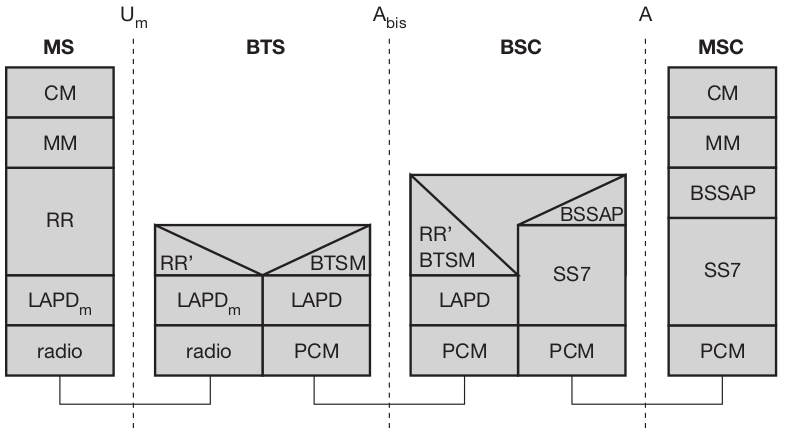
\includegraphics[width=0.8\textwidth]{gsm-protocol-architecture}
	\caption[GSM Protocol architecture.]{Protocol architecture for signaling}
	\label{fig:gsm-protocol-architecture}
\end{figure}



\subsection{MS Protocols}

\subsubsection{Layer 1: Physical Layer}
Layer 1, the \textit{physical layer}, handles all \textit{radio specific} functions.
\begin{itemize}
	\item channel coding
	\item error detection/correction
\end{itemize}

%\subsection*{PCM}
%Data transmission at the physical layer typically uses pulse code modulation (PCM) systems.


\subsubsection{Layer 2: Data Link Layer}
\begin{itemize}
	\item In layer 2, at the \(U_m\) interface, \(\mathbf{LAPD_m}\) has been defined for the purpose of signaling between entities in a \gls{gsm} network.
	\item \(\mathbf{LAPD_m}\) has been derived from link access procedure for the D-channel (LAPD) in ISDN systems, which is a version of HDLC.
	\item \(\mathbf{LAPD_m}\) is a lightweight LAPD because it does not need synchronization flags or checksumming for error detection.
\end{itemize}

%\subsubsection*{Signaling System No. 7 (SS7)} 
%SS7 is used for signaling between an MSC and a BSC. This protocol also transfers all management information between MSCs, HLR, VLRs, AuC, EIR, and OMC. 


\subsubsection{Layer 3: Network Layer}
The network layer in GSM, layer three, comprises several sublayers as shown in Figure \ref{fig:gsm-protocol-architecture}.

\begin{enumerate}
	\item Radio Resource Management (RR)
	\item Mobility Management (MM)
	\item Connection Management (CM)
\end{enumerate}

\subsection{MS to BTS Protocols}

\subsubsection*{RR}
The lowest sublayer is the radio resource management (RR). The main tasks of RR are:
\begin{itemize}
	\item \textit{setup}, \textit{maintenance}, and \textit{release of radio channels}.
	\item RR also directly accesses the physical layer for radio information and offers a reliable connection to the next higher layer.
\end{itemize}

\subsubsection*{MM}
The MM layer is stacked above the RR layer.
 \begin{itemize}
 	\item Mobility management (MM) contains functions for \textit{registration}, \textit{authentication}, \textit{identification}, \textit{location updating}, and the \textit{provision of a TMSI} that replaces the IMSI.
 	\begin{itemize}
 		\item TMSI hides the real identity of an MS user over the air interface.
 		\item TMSI is valid only in the current location area of a VLR.
 	\end{itemize}
 	\item MM offers a reliable connection to the next higher layer.
 \end{itemize}

\subsubsection*{CM}
The CM layer is the topmost layer of the GSM protocol stack. The call management (CM) layer contains three entities: 
\begin{multicols}{2}
	\begin{enumerate}
		\item call control (CC), 
		\item short message service (SMS), and 
		\item supplementary service (SS).
	\end{enumerate}
\end{multicols}

\paragraph*{SMS} allows for message transfer.

\paragraph*{CC} provides a point-to-point connection between two terminals and is used by higher layers for call establishment, call clearing and change of call parameters.

%\subsubsection*{BSSAP}
%An MSC can also control a BSS via a BSS application part (BSSAP).\\
%
%\noindent Additional protocols are used at the \(A_bis\) and \(A\) interfaces. LAPD is used for layer 2 at \(A_bis\), BTSM for BTS management.

\subsection{BSC Protocols}
\begin{itemize}
	\item The BSC uses a different set of protocols after receiving the data from the BTS. 
	\item The \(A_{bis}\) interface is used between the BTS and BSC.
	\item At this level, the radio resources at the lower portion of Layer 3 are changed from the RR to the Base Transceiver Station Management (BTSM). 
	\item The BTS management layer is a relay function at the BTS to the BSC.
\end{itemize}

The RR protocols are responsible for the allocation and reallocation of traffic channels between the MS and the BTS.

To transit from the BSC to the MSC, the BSS mobile application part or the direct application part is used, and SS7 protocols is applied by the relay.

\subsection{MSC Protocols}

\begin{itemize}
	\item At the MSC, starting from the BSC, the information is mapped across the \(A\) interface to the MTP Layers 1 through 3.
	\item Here, Base Station System Management Application Part (BSS MAP) is said to be the equivalent set of radio resources.
	\item The relay process is finished by the layers that are stacked on top of Layer 3 protocols, they are BSS MAP/DTAP, MM, and CM.
	\item This completes the relay process.
	\item To find and connect to the users across the network, MSCs interact using the control-signaling network.
\end{itemize}

%Each GSM MS user is given a HLR that in turn comprises the user’s location and subscribed services. VLR is a separate register that is used to track the location of a user. When the users move out of the HLR covered area, the VLR is notified by the MS to find the location of the user. The VLR in turn, with the help of the control network, signals the HLR of the MS’s new location. With the help of location information contained in the user’s HLR, the MT calls can be routed to the user.

\section{Localization and Calling}
One fundamental feature of the GSM system is the automatic, worldwide localization of users. The system always knows where a user currently is, and the same phone number is valid worldwide. To provide this service, GSM performs periodic location updates even if a user does not use the mobile station (provided that the MS is still logged into the GSM network and is not completely switched off). 

The HLR always contains information about the current location, and the VLR currently responsible for the MS informs the HLR about location changes. As soon as an MS moves into the range of a new VLR (a new location area), the HLR sends all user data needed to the new VLR. \textbf{Changing VLRs with uninterrupted availability of all services is also called roaming}. Roaming can take place within the network of one provider, between two providers in one country, but also between different providers in different countries (international roaming).

\subsection{Localization}
To locate an MS and to address the MS, several numbers are needed:

\subsubsection{MSISDN}
MSISDN is the phone number of a GSM user. It follows the standard for addresses as it is also used in fixed ISDN networks. This number
consists of the:
\begin{itemize}
	\item \textbf{country code} (CC) (e.\ g.\, \texttt{+977 024-123456} with 977 for Nepal)
	\item the \textbf{national destination code (NDC)} (i.\ e.\ , the address of the network provider), and 
	\item the \textbf{subscriber number (SN)}.
\end{itemize}

\subsubsection{IMSI}
 \begin{itemize}
 	\item GSM uses the IMSI for internal unique identification of a subscriber.
 	\item IMSI consists of:
 		\begin{itemize}
 			\item a \textbf{mobile country code (MCC)} (e.\ g.\ , 429 for Nepal), 
 			\item the \textbf{mobile network code (MNC)} (i.\ e.\ , the code of the network provider. e.\ g.\ , 01 for Nepal Telecom, 02 for Ncell), and finally
 			\item the \textbf{mobile subscriber identification number (MSIN)}.
 		\end{itemize}
 \end{itemize}  

\subsubsection{TMSI}

\begin{itemize}
	\item TMSI hides the IMSI to prevent leaking identity of the user signaling over the air interface. 
	\item GSM uses the 4 byte TMSI for local subscriber identification.
	\item TMSI is selected by the current VLR.
	\item TMSI is only valid temporarily and within the location area of the VLR.
	\item VLR may change the TMSI periodically.
\end{itemize}

\subsubsection[MSRN]{Mobile Station Roaming Number (MSRN)}
\begin{itemize}
	\item MSRN is slo a temporary address that hides the identity and location of a subscriber.
	\item The VLR generates this address on request from the MSC, and the address is also stored in the HLR.
	\item MSRN contains:
	\begin{itemize}
		\item the current \textbf{visitor country code (VCC)}, 
		\item the \textbf{visitor national destination code (VNDC)}, 
		\item the identification of the current MSC together with the subscriber number.
	\end{itemize}
\item The MSRN helps the HLR to find a subscriber for an incoming call.
\end{itemize}

\noindent All these numbers are needed to find a subscriber and to maintain the connection with a mobile station. The interesting case is the \textbf{mobile terminated call (MTC)}.

\subsection{Calling}
There are two approaches to call setup:
\begin{itemize}
	\item \textit{Mobile originated call (MOC)}: Mobile subscriber initiates the call.
	\item \textit{Mobile terminated call (MTC)}: Subscriber Receives the call.
\end{itemize}
\subsubsection{MTC}
MTC is a situation in which a station calls a mobile station (the calling station could be outside the GSM network or another mobile station). Figure \ref{fig:mtc-mobile-terminated-call} shows the basic steps needed to connect the calling station with the mobile user. 

%%%%%%%%%%%%%%%%%%%%%%%%%%%%%
%							%
%		FIGURE				%
%							%
%%%%%%%%%%%%%%%%%%%%%%%%%%%%%
\begin{figure}[hb!]
	\centering
	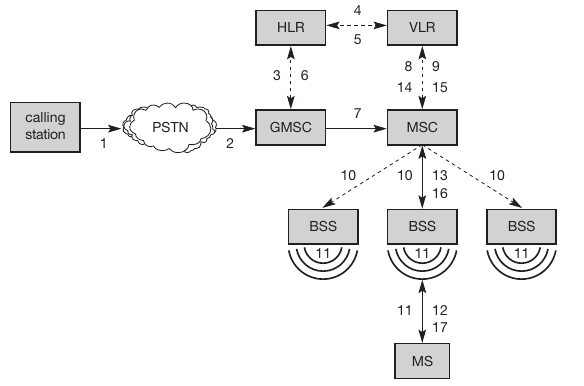
\includegraphics[width=0.8\textwidth]{mtc-mobile-terminated-call}
	\caption{Mobile terminated call (MTC)}
	\label{fig:mtc-mobile-terminated-call}
\end{figure}

Following are the steps involved during MTC:
\begin{steps}
\item A user dials the phone number of a GSM subscriber. 
\item The PSTN forwards the call setup to the GMSC.
\item The GMSC identifies the HLR for the subscriber and signals the call setup to the HLR.
\item The HLR now checks whether the number exists and whether the user has subscribed to the requested services, and requests an MSRN from the current VLR.
\item HLR Receives an MSRN from the VLR.
\item The HLR can determine the MSC responsible for the MS and forwards this information to the GMSC.
\item The GMSC can now forward the call setup request to the MSC indicated.
		\subitem From this point on, the MSC is responsible for all further steps.
\item Requests the current status of the MS from the VLR.
\item Receives the status of the MS.
\item MSC initiates paging in all cells it is responsible for, if the MS is available.
\item The BTSs of all BSSs transmit this paging signal to the MS.
\item MS answers to the BSS.
\item BSS answers to the MSC.
\item The VLR has to perform security checks (set up encryption etc.).
\item The VLR then signals to the MSC to set up a connection.
\item MSC then signals BSS to set up a connection.
\item BSS then signals MS to set up a connection.
\end{steps}




\subsubsection{MOC}
It is much simpler to perform a MOC compared to a MTC (see Figure \ref{fig:moc-mobile-originated-call}). 

Following steps are involved during MOC:

\begin{steps}
	\item The MS transmits a request for a new connection.
	\item The BSS forwards this request to the MSC.
	\item The MSC request VLR to checks if this user is allowed to set up a call with the requested service.\label{itm:Step-3}
	\item VLR confirms request made in \ref{itm:Step-3} and signals to the MSC.
	\item MSC request GMSC for the availability of resources through GSM network.
	\item GMSC then request PSTN for resources.
	\item PSTN responds to GMSC.
	\item GMSC responds back to MSC.
	\item MSC sets up connection with BSS.
	\item BSS and MSC then sets up connection between MS and the fixed network. 
\end{steps}

%%%%%%%%%%%%%%%%%%%%%%%%%%%%%
%							%
%		FIGURE				%
%							%
%%%%%%%%%%%%%%%%%%%%%%%%%%%%%
\begin{figure}[ht!]
	\centering
	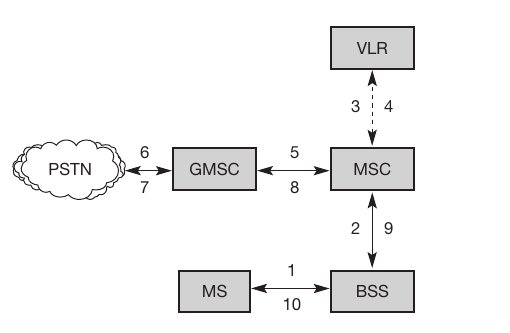
\includegraphics[width=0.8\textwidth]{moc-mobile-originated-call}
	\caption{Mobile originated call (MOC)}\label{fig:moc-mobile-originated-call}
\end{figure}

\begin{framed}
\subsubsection*{\textnp{MOC लाई बुँदागत रुपमा नलेखेर सङ्‍क्षेपमा यस प्रकारले पनि लेख्न सकिन्छ}}
It is much simpler to perform a mobile originated call (MOC) compared to a MTC. The MS transmits a request for a new connection (1), the BSS forwards this request to the MSC (2). The MSC then checks if this user is allowed to set up a call with the requested service (3 and 4) and checks the availability of resources through the GSM network and into the PSTN. If all resources are available, the MSC sets up a connection between the MS and the fixed network.
\end{framed}

\section{Handover}

Cellular systems require \textit{handover} procedures, as single cells do not cover the whole service area, but, e.\ g.\ , only up to 35 km around each antenna on the countryside and some hundred meters in cities. The smaller the cell size and the faster the movement of a mobile station through the cells (up to \(250 km/h\) for GSM), the more handovers of ongoing calls are required. However, a handover should not cause a cut-off, also called call drop. GSM aims at maximum handover duration of \(60 ms\).

\subsection{Basic Reasons For Handover}
There are two basic reasons for a handover:


\subsubsection[Out of Range]{MS moves out of the range of a BTS}
\begin{itemize}
	\item The mobile station moves out of the range of a BTS or a certain antenna of a BTS respectively.
	\item The received \textit{signal level} decreases continuously until it falls below the minimal requirements for communication.
	\item \textit{The error rate} may grow due to interference, the distance to the BTS may be too high
	\item All these effects may diminish the \textit{quality of the radio link} and make radio transmission impossible in the near future.
\end{itemize}
 


\subsubsection[High Traffic]{Too high traffic in one cell}

\begin{itemize}
	\item The wired infrastructure (MSC, BSC) may decide that the \textit{traffic in one cell is too high} and shift some MS to other cells with a lower load (if possible).
	\item Handover may be due to \textit{load balancing}.
\end{itemize}

\subsection{Handover Scenarios}
Figure \ref{fig:gsm-handover} shows four possible handover scenarios in GSM:

\begin{itemize}
	\item \textit{Intra-cell handover}.	
	\item \textit{Inter-cell, intra-BSC handover}
	\item \textit{Inter-BSC, intra-MSC handover}:
	\item \textit{Inter MSC handover}
\end{itemize}

%%%%%%%%%%%%%%%%%%%%%%%%%%%%%
%							%
%		FIGURE				%
%							%
%%%%%%%%%%%%%%%%%%%%%%%%%%%%%
\begin{figure}[ht!]
	\vspace*{0.2cm}
	\centering
	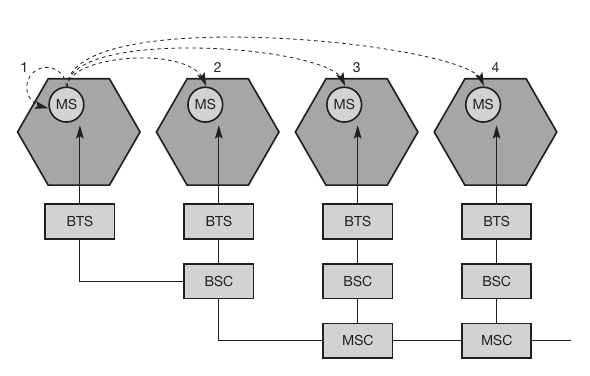
\includegraphics[width=0.8\textwidth]{gsm-handover}
	\caption{Types of handover in GSM}\label{fig:gsm-handover}
\end{figure}

\subsubsection[Intra-cell Handover]{Scenario 1: Intra-cell Handover}
\begin{itemize}
	\item Within a cell, narrow-band interference could make transmission at a certain frequency impossible. 
	\item The BSC could then decide to change the carrier frequency.
\end{itemize}

\subsubsection[Inter-cell, Intra-BSC Handover]{Scenario 2: Inter-cell, Intra-BSC Handover}
\begin{itemize}
	\item This is a typical handover scenario. 
	\item The mobile station moves from one cell to another, but stays within the control of the same BSC. 
	\item The BSC then performs a handover, assigns a new radio channel in the new cell and releases the old one.
\end{itemize}


\subsubsection[Inter-BSC, Intra-MSC Handover]{Scenario 3: Inter-BSC, Intra-MSC Handover}
\begin{itemize}
	\item As a BSC only controls a limited number of cells; GSM also has to perform handovers between cells controlled by different BSCs.
	\item This handover then has to be controlled by the MSC.
\end{itemize}

\subsubsection[Inter MSC handover]{Scenario 4: Inter MSC handover}
\begin{itemize}
	\item A handover could be required between two cells belonging to different MSCs. 
	\item Now both MSCs perform the handover together.
\end{itemize}


\noindent Figure \ref{fig:intra-msc-handover} shows the typical signal flow during an inter-BSC, intra-MSC handover. 

\begin{itemize}
	\item The MS sends its periodic measurements reports, the $ BTS_{old} $ forwards these reports to the $ BSC_{old} $ together with its own measurements. 
	\item Based on these values and, the $ BSC_{old} $ may decide to perform a handover and sends the message \verb*|HO_required| to the MSC. 
	\item The task of the MSC then comprises the request of the resources needed for the handover from the new BSC, $ BSC_{new} $. 
	\item This BSC checks if enough resources  are available and activates a physical channel at the $ BTS_{new} $ to prepare for the arrival of the MS.
	\item The $ BTS_{new} $ acknowledges the successful channel activation, $ BSC_{new} $ acknowledges the handover request. 
	\item The MSC then issues a handover command that is forwarded to the MS. 
	\item The MS now breaks its old radio link and accesses the new BTS. 
	\item The next steps include the establishment of the link (this includes layer two link establishment and handover complete messages from the MS). 
	\item Basically, the MS has then finished the handover, but it is important to release the resources at the old BSC and BTS and to signal the successful handover using the handover and clear complete messages as shown.
\end{itemize}



%%%%%%%%%%%%%%%%%%%%%%%%%%%%%
%							%
%		FIGURE				%
%							%
%%%%%%%%%%%%%%%%%%%%%%%%%%%%%

\begin{figure}[ht!]
	\centering
	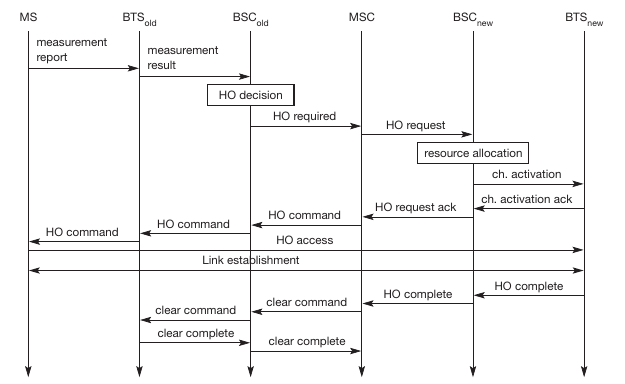
\includegraphics[width=0.8\textwidth]{intra-msc-handover}
	\caption{Intra-MSC handover}\label{fig:intra-msc-handover}
\end{figure}



\section{Security}
GSM offers several security services using confidential information stored in the AuC and in the individual SIM (which is plugged into an arbitrary MS). The SIM stores personal, secret data and is protected with a PIN against unauthorized use. (For example, the secret key \(K_i\) used for authentication and encryption procedures is stored in the SIM.) 

\subsection{GSM Security Services}
The security services offered by GSM are:
\begin{itemize}
	\item \textit{Access control and authentication}
	\item \textit{Confidentiality}
	\item \textit{Anonymity}
\end{itemize}

\subsubsection{Access Control and Authentication}
\begin{itemize}
	\item The first step includes the authentication of a valid user for the SIM. The user needs a secret PIN to access the SIM.
	\item The next step is the subscriber authentication. 
	\item This step is based on a challenge-response scheme as presented in Section \ref{sec:challenge-response}.
\end{itemize}

\subsubsection{Confidentiality}
\begin{itemize}
	\item All user-related data is encrypted. 
	\item After authentication, BTS and MS apply encryption to voice, data, and signaling as shown in Section \ref{sec:encryption}. 
	\item This confidentiality exists only between MS and BTS, but it does not exist end-to-end or within the whole fixed GSM/telephone network.
\end{itemize}


\subsubsection{Anonymity}
\begin{itemize}
	\item To provide user anonymity, all data is encrypted before transmission, and user identifiers are not used over the air.
	\item Instead, GSM transmits a temporary identifier (TMSI), which is newly assigned by the VLR after each location update.
	\item Additionally, the VLR can change the TMSI at any time.
\end{itemize}

\noindent Three algorithms have been specified to provide security services in GSM:
\begin{itemize}
	\item Algorithm $ A3 $ is used for \textit{authentication},
	\item $ A5 $ for \textit{encryption}, and
	\item $ A8 $ for the \textit{generation of a cipher key}.
\end{itemize}

\noindent In the GSM standard only algorithm $ A5 $ was publicly available, whereas $ A3 $ and $ A8 $ were secret, but standardized with open interfaces. Both $ A3 $ and $ A8 $ are no longer secret, but were published on the internet in 1998. 

Algorithms $ A3 $ and $ A8 $ (or their replacements) are located on the SIM and in the AuC and can be proprietary. Only $ A5 $ which is implemented in the devices has to be identical for all providers.

\subsection{Authentication}\label{sec:challenge-response}
Before a subscriber can use any service from the GSM network, he or she must be authenticated. Authentication is based on the SIM, which stores the: 
%\begin{multicols}{2}
\begin{enumerate}
	\item \textbf{individual authentication key} $ K_i $, 
	\item \textbf{user identification IMSI}, and 
	\item algorithm used for authentication \textbf{A3}. 
\end{enumerate}
%\end{multicols}



\noindent Authentication uses a challenge-response method:
\begin{steps}
	\item The access control AC generates a random number \textbf{RAND} as challenge, and 
	\item the SIM within the MS answers with \textbf{SRES} (signed response) as response (see Figure \ref{fig:subscriber-auth}). 
	\item The AuC performs the basic generation of random values $ RAND $, signed responses $ SRES $, and cipher keys $ K_c $ for each IMSI, and then forwards this information to the HLR. 
	\item The current VLR requests the appropriate values for $ RAND $, $ SRES $, and $ K_c $ from the HLR.
	\item The VLR sends the random value $ RAND $ to the SIM. 
	\item Both sides, network and subscriber module, perform the same operation with $ RAND $ and the key $ K_i $, called $ A3 $. 
	\item The MS sends back the $ SRES $ generated by the SIM; the VLR can now compare both values. 
	\item If they are the same, the VLR accepts the subscriber, otherwise the subscriber is rejected.
\end{steps}



%%%%%%%%%%%%%%%%%%%%%%%%%%%%%
%							%
%		FIGURE				%
%							%
%%%%%%%%%%%%%%%%%%%%%%%%%%%%%

\begin{figure}[ht!]
	\vspace*{0.2cm}
	\centering
	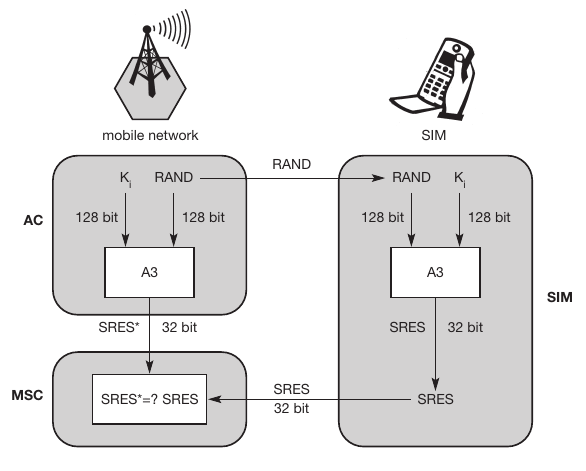
\includegraphics[width=0.8\textwidth]{subscriber-auth}
	\caption{Subscriber authentication}\label{fig:subscriber-auth}
\end{figure}


\subsection{Encryption}\label{sec:encryption}
To ensure privacy, all messages containing user-related information are encrypted in GSM over the air interface. 

\begin{itemize}
	\item After authentication, MS and BSS can start using encryption by applying the cipher key $ K_c $. 
	\item $ K_c $ is generated using the individual key $ K_i $ and a random value by applying the algorithm $ A8 $. 
	\item SIM in the MS and the network both calculate the same $ K_c $ based on the random value RAND. 
	\item The key $ K_c $ itself is not transmitted over the air interface.
\end{itemize}
%%%%%%%%%%%%%%%%%%%%%%%%%%%%%
%							%
%		FIGURE				%
%							%
%%%%%%%%%%%%%%%%%%%%%%%%%%%%%

\begin{figure}[ht!]
	\centering
	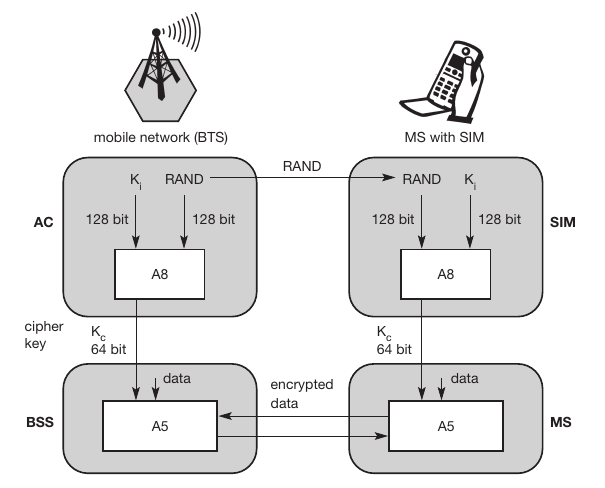
\includegraphics[width=0.8\textwidth]{data-encryption}
	\caption{Data encryption}\label{fig:data-encryption}
\end{figure}

MS and BTS can now encrypt and decrypt data using the algorithm A5 and the cipher key $ K_c $. As Figure \ref{fig:data-encryption} shows, $ K_c $ should be a 64 bit key — which is not very strong, but is at least a good protection against simple eavesdropping.


\newpage
\section{GPRS}
The general packet radio service (GPRS) provides packet mode transfer for applications that exhibit traffic patterns such as frequent transmission of small volumes (e.\ g.\ , typical web requests) or infrequent transmissions of small or medium volumes (e.\ g.\ , typical
web responses) according to the requirement specification. 

The key element of GPRS technology is that it uses packet switched data rather than circuit switched data, and this technique makes much more efficient use of the available capacity. The data is split into packets and tags inserted into the packet to provide the destination address. Packets from several sources can then be transmitted over the link.

\subsection*{Goal}
The provision of a more efficient and, thus, cheaper packet transfer service for typical internet applications that usually rely solely on packet transfer. 

\subsection*{Benefit}
The main benefit for users of GPRS is the `always on’ characteristic — no connection has to be set up prior to data transfer.

\subsection*{Motivation for Development} 
GPRS was driven by the tremendous success of the packet-oriented internet, and by the new traffic models and applications.


\subsection{GPRS System Architecture}
%The GPRS architecture introduces two new network elements, which are called \textbf{GPRS support nodes (GSN)} and \textbf{serving GPRS support node (SGSN)} 

\subsubsection[GSN]{GPRS Support Node (GSN)}
\textbf{GPRS support nodes (GSN)} and are in fact routers. All GSNs are integrated into the standard GSM architecture, and many new interfaces have been defined (see Figure \ref{fig:gprs-arch}). 

\subsubsection[GGSN]{Gateway GPRS Support Node (GGSN)}
The \textbf{gateway GPRS support node (GGSN)} is the interworking unit between the GPRS network and external \textbf{packet data networks (PDN)}. This node
\begin{itemize}
	\item contains routing information for GPRS users, 
	\item performs address conversion, and 
	\item tunnels data to a user via encapsulation.
\end{itemize}
 The GGSN is connected to external networks (e.\ g.\ , IP or X.25) via the $ G_i $ interface and transfers packets to the SGSN via an IP-based GPRS backbone network ($ G_n $ interface).

\subsubsection[SGSN]{Serving GPRS Support Node}
The \textbf{serving GPRS support node (SGSN)} which supports the MS via the $ G_b $ interface. The SGSN, for example, 
\begin{itemize}
	\item requests user addresses from the \textbf{GPRS register (GR)}, 
	\item keeps track of the individual MSs' location, is responsible for collecting billing information (e.\ g.\ , counting bytes), and \item performs several security functions such as access control.
\end{itemize}


 \noindent The SGSN is connected to a BSC via frame relay and is basically on the same hierarchy level as an MSC. The GR, which is typically a part of the HLR, stores all GPRS-relevant data. GGSNs and SGSNs can be compared with home and foreign agents, respectively, in a mobile IP network.
 
%%%%%%%%%%%%%%%%%%%%%%%%%%%%%%%%%%%%%%%%%%%%%
%											%
%				Figure						%
%											%
%%%%%%%%%%%%%%%%%%%%%%%%%%%%%%%%%%%%%%%%%%%%%
\begin{figure}[H]
	\centering
	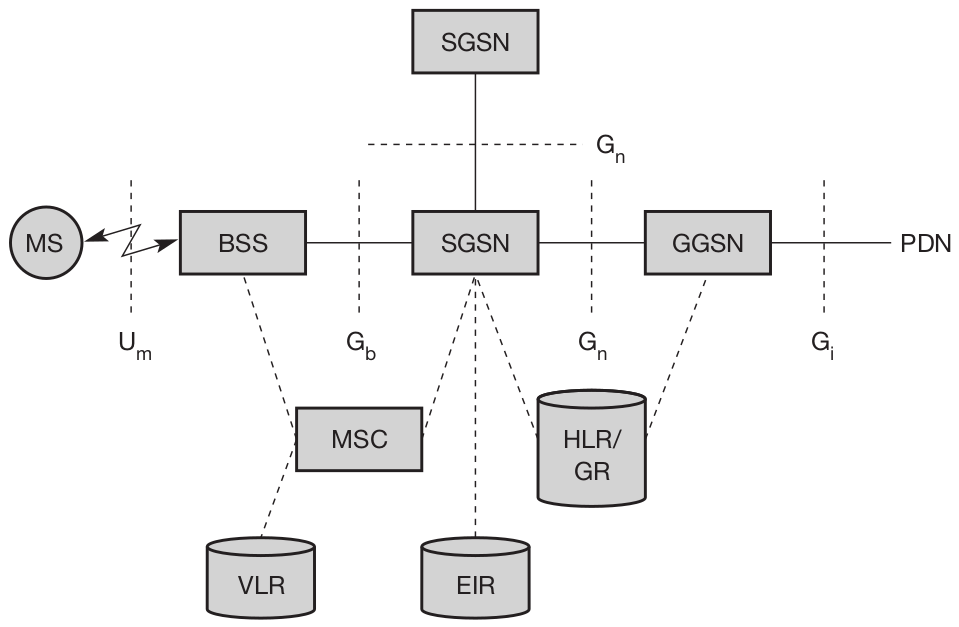
\includegraphics[width=0.8\textwidth]{gprs-arch}
	\caption{GPRS architecture reference model}\label{fig:gprs-arch}
\end{figure}
%-----------------------FIGURE END------------------------
As shown in Figure \ref{fig:gprs-arch}, packet data is transmitted from a PDN, via the GGSN and SGSN directly to the BSS and finally to the MS. The MSC, which is responsible for data transport in the traditional circuit-switched GSM, is only used for signaling in the GPRS scenario.


Before sending any data over the GPRS network, 
\begin{itemize}
	\item An MS must attach to it, following the procedures of the \textbf{mobility management}. 
	\item The attachment procedure includes assigning a temporal identifier, called a \textbf{temporary logical link identity (TLLI)}, and a \textbf{ciphering key sequence number (CKSN)} for data encryption. 
	\item For each MS, a \textbf{GPRS context} is set up and stored in the MS and in the corresponding SGSN. This context comprises:
	\begin{itemize}
		\item the status of the MS (which can be ready, idle, or standby), 
		\item the CKSN, 
		\item a flag indicating if compression is used, and 
		\item routing data (TLLI, the routing area RA, a cell identifier, and a packet data channel, PDCH, identifier)
	\end{itemize}
 \item Besides attaching and detaching, mobility management also comprises functions for:
 	\begin{itemize}
 		\item authentication, 
 		\item location management, and 
 		\item ciphering.
 	\end{itemize} 
 \item In \textbf{idle} mode an MS is not reachable and all context is deleted.
 \item In the \textbf{standby} state only movement across routing areas is updated to the SGSN but not changes of the cell.
\end{itemize}

Permanent updating would waste battery power, no updating would require system-wide paging. The update procedure in standby mode is a compromise. Only in the \textbf{ready} state every movement of the MS is indicated to the SGSN.



\section{UMTS}
The Universal Mobile Telecommunications System (UMTS) is a third generation mobile cellular system for networks based on the GSM standard. Developed and maintained by the 3GPP ($ 3^{rd} $ Generation Partnership Project), UMTS is a component of the Standard International Union all IMT-2000 telecommunications and compares it with the standard set for CDMA2000 networks based on competition cdmaOne technology. UMTS uses wideband code division multiple access (W-CDMA) radio access technology to provide greater spectral efficiency and bandwidth mobile network operators.

\subsection{UMTS System Architecture}

Figure \ref{fig:umts-components} shows the very simplified UMTS reference architecture.

\begin{itemize}
	\item The \textbf{UTRA network (UTRAN)} handles cell level mobility and comprises several \textbf{radio network subsystems (RNS)}. 
	\item The functions of the RNS include radio channel ciphering and deciphering, handover control, radio resource management etc.
	\item The UTRAN is connected to the \textbf{user equipment (UE)} via the radio interface $ U_u $ (which is comparable to the $ U_m $ interface in GSM) via the $ I_u $ interface (which is similar to the $ A $ interface in GSM), UTRAN communicates with the \textbf{core network (CN)}. 
	\item The CN contains functions	for inter-system handover, gateways to other networks (fixed or wireless), and performs location management if there is no dedicated connection between UE and UTRAN.
\end{itemize}

%%%%%%%%%%%%%%%%%%%%%%%%%%%%%%%%%%%%%%%%%%%%%
%											%
%				Figure						%
%											%
%%%%%%%%%%%%%%%%%%%%%%%%%%%%%%%%%%%%%%%%%%%%%
\begin{figure}[hpt]
	\centering
	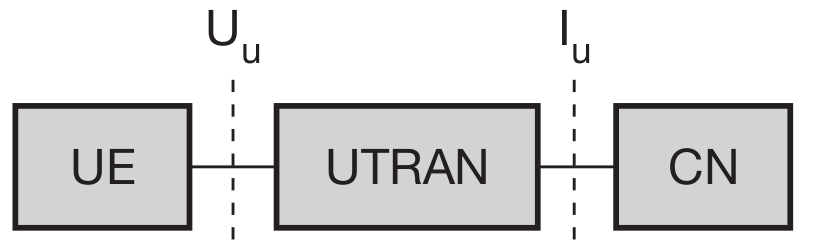
\includegraphics[width=0.6\textwidth]{umts-components}
	\caption{Main components of the UMTS reference architecture}\label{fig:umts-components}
\end{figure}
%-----------------------FIGURE END------------------------



The UMTS network architecture can be divided following elements. Figure \ref{fig:umts-architecture} shows the UMTS architecture.




%%%%%%%%%%%%%%%%%%%%%%%%%%%%%%%%%%%%%%%%%%%%%
%											%
%				Figure						%
%											%
%%%%%%%%%%%%%%%%%%%%%%%%%%%%%%%%%%%%%%%%%%%%%
\begin{figure}[hpt]
	\centering
	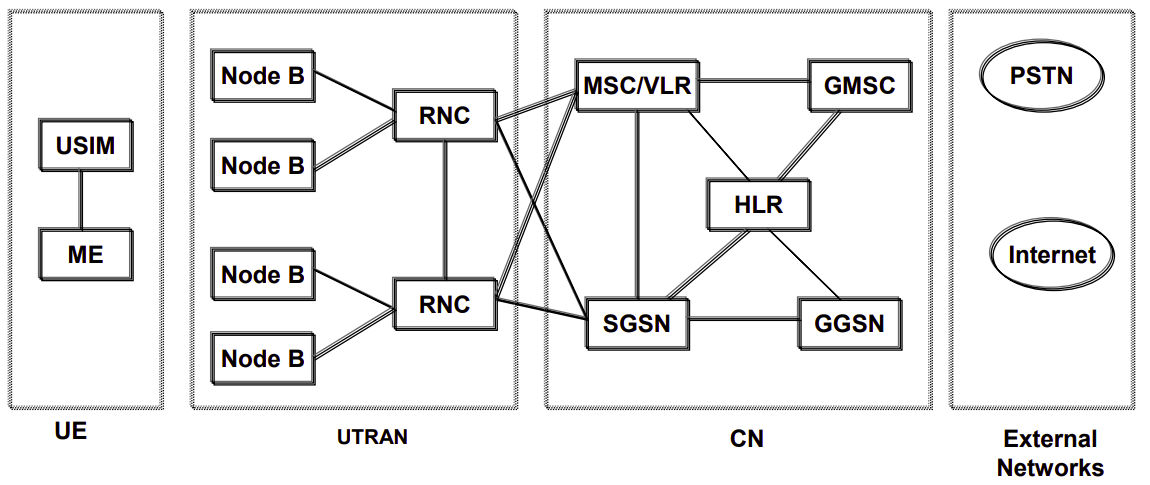
\includegraphics[width=0.9\textwidth]{umts-architecture}
	\caption{UMTS architecture}\label{fig:umts-architecture}
\end{figure}
%-----------------------FIGURE END------------------------
UMTS system composed of three main subsystems:
\begin{itemize}
	\item \textbf{UE (User Equipment)} that interfaces with the user
	\item \textbf{UTRAN (UMTS Terrestrial Radio Access Network)} handles all radio related functionality — WCDMA is radio interface standard here.
	\item \textbf{CN (Core Network)} is responsible for transport functions such as	switching and routing calls and data, tracking users.
\end{itemize}

\subsubsection{UE}
It includes:
\begin{itemize}
	\item ME (Mobile Equipment) and
	\item USIM (UMTS Subscriber Identity Module)
\end{itemize}

\paragraph{ME}
ME is the single or multimode terminal used for radio communication

\paragraph{USIM}
USIM is a smart card that holds the subscriber identity, subscribed services, authentication and encryption keys. 


\subsubsection{UTRAN}
It includes:
\begin{itemize}
	\item Node B
	\item RNC (Radio Network Controller)
\end{itemize}

\paragraph{Node B}
 Node B is equivalent to BTS in GSM/GPRS.
 \begin{itemize}
 	\item It performs the air interface processing (channel coding, rate adaptation, spreading, synchronization, power control).
 	\item It can operate a group of antennas/radios. 
 \end{itemize}

\paragraph{RNC}
RNC is equivalent to GSM BSC.
\begin{itemize}
	\item It is responsible for radio resource management and control of the Node Bs.
	\item Also responsible for handoff decisions, congestion control, power control, encryption, admission control, protocol conversion, etc. 
\end{itemize}


\subsubsection{CN}

\paragraph{HLR}
\begin{itemize}
	\item HLR is a database located in the user’s home system that stores the master copy of the user’s service profile.
	\item The HLR also stores the UE location on the level of MSC and SGSN.
\end{itemize}

\paragraph{3G MSC / VLR}
\begin{itemize}
	\item MSC/VLR are Switch and database that serves the UE in its current location for Circuit Switched (CS) services. 
	\item The MSC function is used to switch the CS	transactions, and VLR function holds a copy of the visiting user’s service
	profile, as well as more precise information on the UE’s location within the serving system
\end{itemize}

\paragraph{3G GMSC}
\begin{itemize}
	\item GMSC is a switch at the point where UMTS is connected to external CS networks. 
	\item All incoming and outgoing CS connections go through GMSC.
\end{itemize}

\paragraph{3G SGSN}
\begin{itemize}
	\item It is similar to that of MSC / VLR but is used for Packet Switched (PS) services.
	\item The part of the network that is accessed via the SGSN is often referred to as	the PS domain. 
	\item Upgrade version of serving GPRS support node.
\end{itemize}

\paragraph{3G GGSN}
\begin{itemize}
	\item GGSN Functionality is close to that of GMSC but is in the relation to PS services.
	\item Upgraded version of gateway GPRS support Node. 
\end{itemize}

\noindent The Core Network (CN) and the Interface $ I_u $ are separated into two logical domains:

\begin{enumerate}
	\item \textbf{Circuit Switched Domain (CSD)}
	\begin{itemize}
		\item Circuit switched service including signaling
		\item Resource reservation at connection setup
		\item 3G versions of GSM components (MSC, GMSC, VLR, HLR)
		\item $ I_u$CS
	\end{itemize}
	
	\item \textbf{Packet Switched Domain (PSD)}
	\begin{itemize}
		\item Handles all packet data services
		\item 3G versions of GPRS components (SGSN, GGSN)
		\item $ I_u $PS
	\end{itemize}

\end{enumerate}
%https://www.electronics-notes.com/articles/connectivity/3g-umts/network-architecture.php
%\begin{itemize}
%	\item \textbf{User Equipment (UE)}: The User Equipment or UE is the name given to what was previous termed the mobile, or cellphone. The new name was chosen because the considerably greater functionality that the UE could have. It could also be anything between a mobile phone used for talking to a data terminal attached to a computer with no voice capability.
%	
%	\item \textbf{Radio Network Subsystem (RNS)}: The RNS also known as the UMTS Radio Access Network, UTRAN, is the equivalent of the previous Base Station Subsystem or BSS in GSM. It provides and manages the air interface fort he overall network.
%	
%	\item \textbf{Core Network}: The core network provides all the central processing and management for the system. It is the equivalent of the GSM Network Switching Subsystem or NSS.
%\end{itemize}
%
%The core network is then the overall entity that interfaces to external networks including the public phone network and other cellular telecommunications networks.

%\subsubsection*{User Equipment, UE}
%The USER Equipment or UE is a major element of the overall 3G UMTS network architecture. It forms the final interface with the user. In view of the far greater number of applications and facilities that it can perform, the decision was made to call it a user equipment rather than a mobile. However it is essentially the handset (in the broadest terminology), although having access to much higher speed data communications, it can be much more versatile, containing many more applications. It consists of a variety of different elements including RF circuitry, processing, antenna, battery, etc.
%
%There are a number of elements within the UE that can be described separately:
%
%\begin{itemize}
%	\item UE RF circuitry:   The RF areas handle all elements of the signal, both for the receiver and for the transmitter. One of the major challenges for the RF power amplifier was to reduce the power consumption. The form of modulation used for W-CDMA requires the use of a linear amplifier. These inherently take more current than non linear amplifiers which can be used for the form of modulation used on GSM. Accordingly to maintain battery life, measures were introduced into many of the designs to ensure the optimum efficiency.
%	
%	\item Baseband processing:   The base-band signal processing consists mainly of digital circuitry. This is considerably more complicated than that used in phones for previous generations. Again this has been optimised to reduce the current consumption as far as possible.
%	
%	\item Battery:   While current consumption has been minimised as far as possible within the circuitry of the phone, there has been an increase in current drain on the battery. With users expecting the same lifetime between charging batteries as experienced on the previous generation phones, this has necessitated the use of new and improved battery technology. Now Lithium Ion (Li-ion) batteries are used. These phones to remain small and relatively light while still retaining or even improving the overall life between charges.
%	
%	\item Universal Subscriber Identity Module, USIM:   The UE also contains a SIM card, although in the case of UMTS it is termed a USIM (Universal Subscriber Identity Module). This is a more advanced version of the SIM card used in GSM and other systems, but embodies the same types of information. It contains the International Mobile Subscriber Identity number (IMSI) as well as the Mobile Station International ISDN Number (MSISDN). Other information that the USIM holds includes the preferred language to enable the correct language information to be displayed, especially when roaming, and a list of preferred and prohibited Public Land Mobile Networks (PLMN).
%	
%	\item The USIM also contains a short message storage area that allows messages to stay with the user even when the phone is changed. Similarly "phone book" numbers and call information of the numbers of incoming and outgoing calls are stored.
%\end{itemize}
%
%The UE can take a variety of forms, although the most common format is still a version of a "mobile phone" although having many data capabilities. Other broadband dongles are also being widely used.
%



\section{LTE}
\subsection{Long Term Evolution}
LTE stands for Long Term Evolution and is a registered trademark owned by ETSI (European Telecommunications Standards Institute) for the wireless data communications technology and a development of the GSM/UMTS standards.

LTE was the 4G successor to the 3G UMTS system which was developed to provide a further evolution of the mobile telecommunications system available.

Providing much higher data speeds and greatly improved performance as well as lower operating costs, the scheme started to be deployed in its basic form around 2008.

Initial deployments gave little improvement over 3G HSPA and were sometimes dubbed 3.5G or 3.99G, but soon the full capability of LTE was realized it provided a full 4G level of performance.

The first deployments were simply known as LTE, but later deployments were designated 4G LTE Advanced and later still 4G LTE Pro.

Not only was the radio access network improved for 4G LTE, but the network architecture was overhauled enabling lower latency and much better interconnectivity between elements of the radio access network, RAN.


LTE is commonly marketed as 4G LTE \& Advance 4G, but it does not meet the technical criteria of a 4G wireless service.	

\subsection{4G}
4G is a collection of fourth generation cellular data technologies. It succeeds 3G and is also called “IMT-Advanced,” or “International Mobile Telecommunications Advanced.”

All 4G standards must conform to a set of specifications created by the International Telecommunications Union. For example, all 4G technologies are required to provide peak data transfer rates of at least 100 Mbps. While actual download and upload speeds may vary based on signal strength and wireless interference, 4G data transfer rates can actually surpass those of cable modem and DSL connections.

Like 3G, there is no single 4G standard. Instead, different cellular providers use different technologies that conform to the 4G requirements.

4G advantages:
\begin{itemize}
	\item high spectral efficiency;
	\item very low latency;
	\item supports variable bandwidths;
	\item simple protocol architecture;
	\item compatibility and interworking with earlier 3GPP releases;
	\item Frequency division duplex (FDD) and time division duplex (TDD) within a single radio access technology;
	\item efficient multicast/broadcast.
\end{itemize}


	\subsection{5G}
	
%The 5G mobile communications system provides a far higher level of performance than the previous generations of mobile communications systems.
%
%The new 5G technology is not just the next version of mobile communications, evolving from 1G to 2G, 3G, 4G, but it provides a new approach giving ubiquitous connectivity.
%
%5G is able to provide much greater flexibility and therefore it is able to support a much wider range of applications, from low data rate Internet of Things requirements through to very fast data rate and very low latency applications.

5G is the 5th generation mobile network. It is a new global wireless standard after 1G, 2G, 3G, and 4G networks. 5G enables a new kind of network that is designed to connect virtually everyone and everything together including machines, objects, and devices.

5G wireless technology is meant to deliver higher multi-Gbps peak data speeds, ultra low latency, more reliability, massive network capacity, increased availability, and a more uniform user experience to more users. Higher performance and improved efficiency empower new user experiences and connects new industries.

5G is based on OFDM (Orthogonal frequency-division multiplexing), a method of modulating a digital signal across several different channels to reduce interference. 5G uses 5G NR air interface alongside OFDM principles. 5G also uses wider bandwidth technologies such as sub-6 GHz and mmWave.

5G will bring wider bandwidths by expanding the usage of spectrum resources, from sub-3 GHz used in 4G to 100 GHz and beyond. 5G can operate in both lower bands (e.\ g.\ , sub-6 GHz) as well as mmWave (e.\ g.\ , 24 GHz and up), which will bring extreme capacity, multi-Gbps throughput, and low latency.

5G is designed to not only deliver faster, better mobile broadband services compared to 4G LTE, but can also expand into new service areas such as mission-critical communications and connecting the massive IoT. This is enabled by many new 5G NR air interface design techniques, such as a new self-contained TDD subframe design


\subsubsection*{Applications of 5G}
5G is used across three main types of connected services, including:
\begin{itemize}
	 \item enhanced mobile broadband, 
	 \item mission-critical communications, and 
	 \item the massive IoT. 
\end{itemize}
A defining capability of 5G is that it is designed for forward compatibility—the ability to flexibly support future services that are unknown today.

5G is designed to deliver peak data rates up to 20 Gbps based on IMT-2020 requirements.


5G technology has developed rapidly. The first real deployments went live in 2019, and further deployments soon followed. Although there were some teething issues, many noticed a significant increase in speed.





